\documentclass[border=6pt]{standalone}
\usepackage{amsmath,amssymb}
\usepackage{tikz}
\usetikzlibrary{arrows.meta,positioning,shadows,calc}
\begin{document}
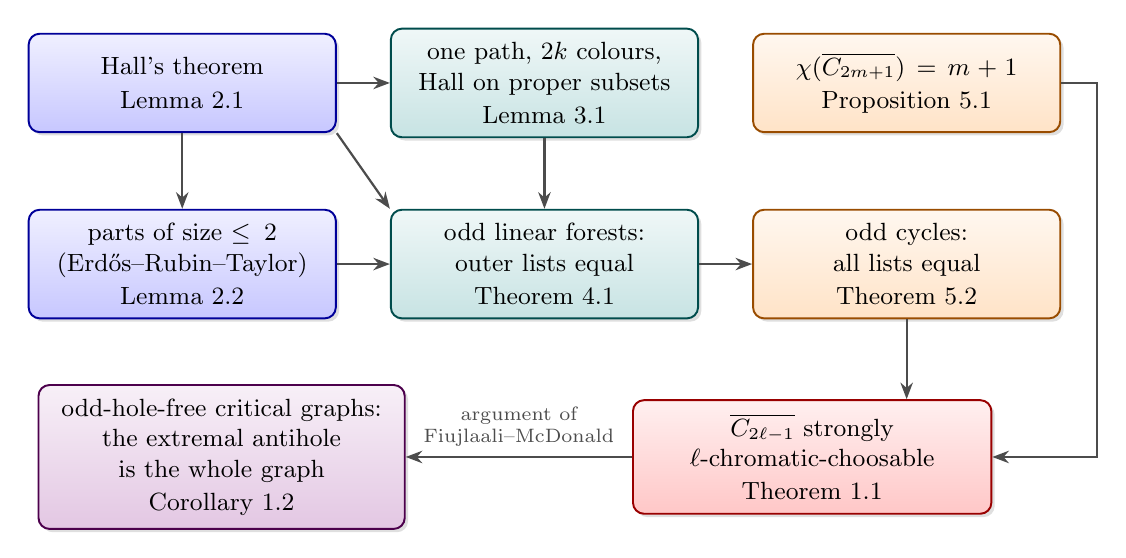
\begin{tikzpicture}[
  box/.style={draw=#1!60!black,line width=0.7pt,rounded corners=4pt,
    top color=#1!6,bottom color=#1!22,drop shadow={opacity=0.25,shadow xshift=1.2pt,shadow yshift=-1.2pt},
    align=center,font=\small,inner sep=5pt,minimum height=1.25cm,text width=3.55cm},
  arr/.style={-{Stealth[length=6pt]},line width=0.8pt,black!70},
  lab/.style={font=\scriptsize,align=center,black!70}]
\node[box=blue] (hall) at (0,0) {Hall's theorem\\[1pt] Lemma 2.1};
\node[box=blue] (ert) at (0,-2.3) {parts of size $\le2$\\ (Erd\H{o}s--Rubin--Taylor)\\[1pt] Lemma 2.2};
\node[box=teal] (key) at (4.6,0) {one path, $2k$ colours,\\ Hall on proper subsets\\[1pt] Lemma 3.1};
\node[box=teal] (path) at (4.6,-2.3) {odd linear forests:\\ outer lists equal\\[1pt] Theorem 4.1};
\node[box=orange] (cyc) at (9.2,-2.3) {odd cycles:\\ all lists equal\\[1pt] Theorem 5.2};
\node[box=orange] (chi) at (9.2,0) {$\chi(\overline{C_{2m+1}})=m+1$\\[1pt] Proposition 5.1};
\node[box=red,text width=4.2cm] (main) at (8.0,-4.75) {$\overline{C_{2\ell-1}}$ strongly\\ $\ell$-chromatic-choosable\\[1pt] Theorem 1.1};
\node[box=violet,text width=4.3cm] (cor) at (0.5,-4.75) {odd-hole-free critical graphs:\\ the extremal antihole\\ is the whole graph\\[1pt] Corollary 1.2};
\draw[arr] (hall) -- (ert);
\draw[arr] (hall) -- (key);
\draw[arr] (hall.south east) -- (path.north west);
\draw[arr] (ert) -- (path);
\draw[arr] (key) -- (path);
\draw[arr] (path) -- (cyc);
\draw[arr] (cyc.south) -- (cyc.south |- main.north);
\draw[arr] (chi.east) -- ++(0.45,0) |- (main.east);
\draw[arr] (main) -- node[lab,above]{argument of\\ Fiujlaali--McDonald} (cor);
\end{tikzpicture}
\end{document}
